\documentclass[12pt]{article}

\usepackage{amssymb}
\usepackage{amsmath}
\usepackage{bm}
\usepackage{dsfont}
\usepackage[margin=1in]{geometry}
\usepackage[font=scriptsize]{caption}
\usepackage{dsfont}
\usepackage{amsmath}
\usepackage{graphicx}
\usepackage{bm}
\newcommand{\m}[1]{\mathbf{\bm{#1}}}
\newcommand{\R}{I\hspace{-4.4pt}R}
\newcommand{\bc}[1]{\textcolor{blue}{\mathbf{#1}}}
\newcommand{\ind}{\mathds{1}}
\newcommand{\m}[1]{\mathbf{\bm{#1}}}
\newcommand{\R}{I\hspace{-4.4pt}R}

% \setlength\parindent{0pt}


\begin{document}

\begin{Large}
\noindent Extreme value comparison of CanCM4 simulations and observations
\end{Large}
% A Bayesian hierarchical model for CanCM4 climate simulations, with an exploration of estimating the extremal index in the hierarchical setting, and a comparison between climate simulations and observations from a gridded product

\section{Introduction}
\label{intro}



Extreme value theory provides the framework for analyzing the stochastic behavior of a process at very large (small) values. This entails calculating the probability distribution of the maximum (minimum) of a sequence of random variabes. 

Equivalently, extreme value analyses study the tails of probability distributions associated with some data generating mechanism. 

In extreme value analyses, a primary interest is to understand 

The standard approach is to appeal to asymtoptic arguments.

We can calculate useful quantities such as return levels.

This allows us to extrapolate beyond the span of historical data.


We compare three types of climate model simulations 

The Fourth Generation Atmospheric General Circulation Model (CanCM4) from Canada 

Decadal, historical, and control runs are used to obtain precipitation and temperature over California and the U.S. We have observational data from Ed Maurer. We will consider two 10-year periods: 1962--1971 and 1990--1999. We will also split these into winter months (December, January, Februrary) and summer months (June, July, August). Precipitation in summer is not analyzed.
\bigskip

Purpose of the univariate analysis?
\bigskip

Details on the differences between decadal, historical, and control runs.
\bigskip

Precipitation based on the observations is summed. Precipitation from the climate model is computed with a weighted sum, based on the number of locations in the observation product.
\bigskip

Description of data processing
\bigskip

Picture of the locations CanCM4/Obs produces
\bigskip

Time-series plot of the variables
\bigskip

\begin{figure}
\begin{center}
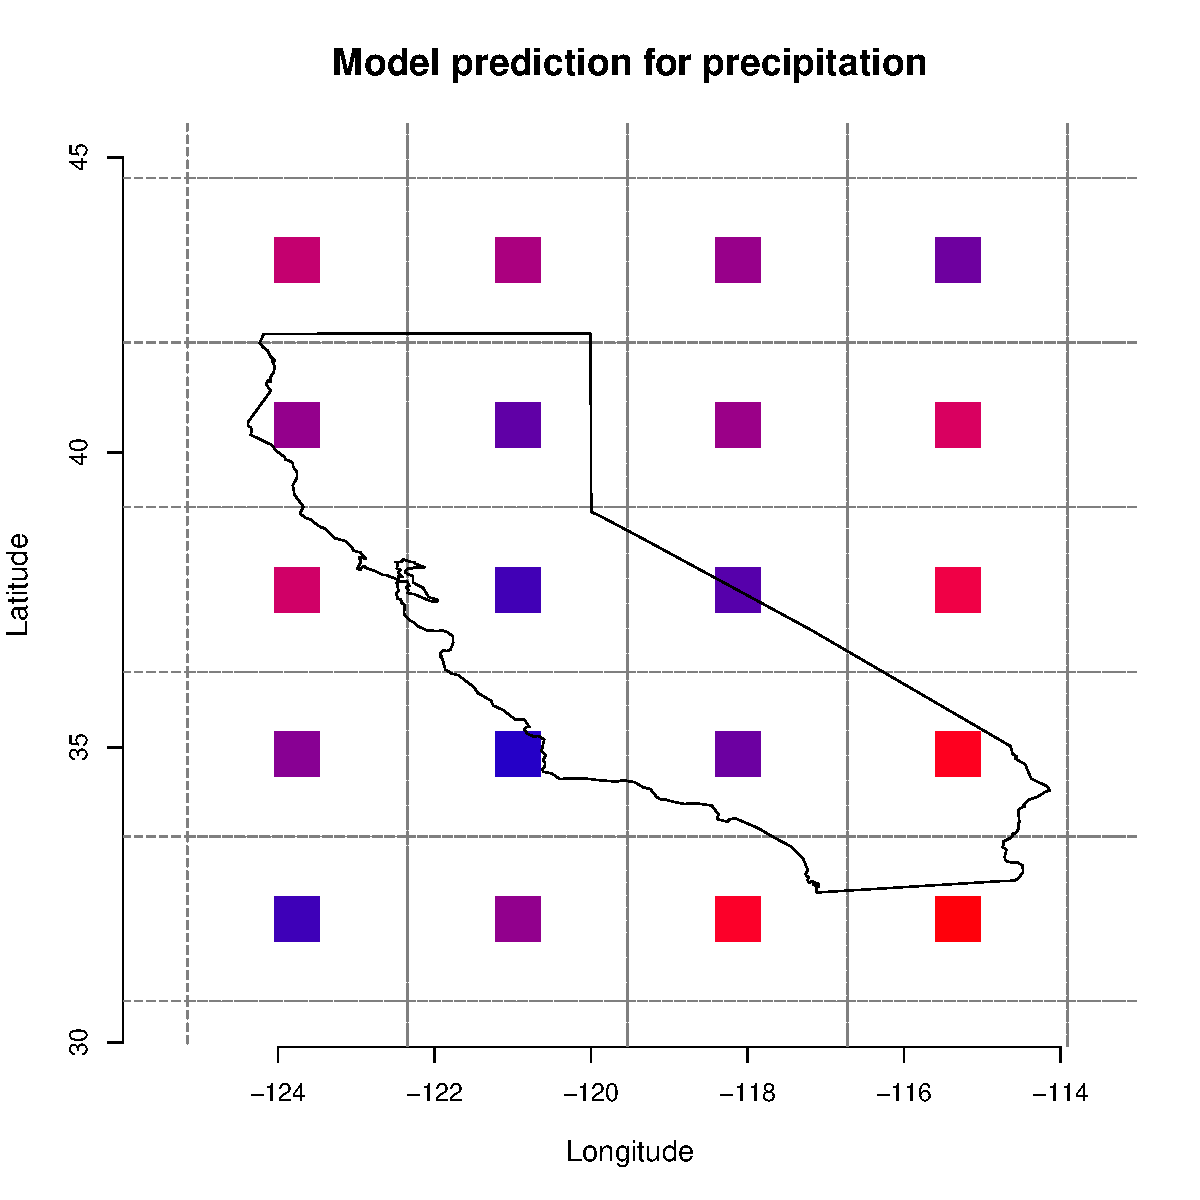
\includegraphics[scale=0.26]{/home/mickey/files/repos/stat_clim_evt_repo/figs/cal_mod_box1.pdf}
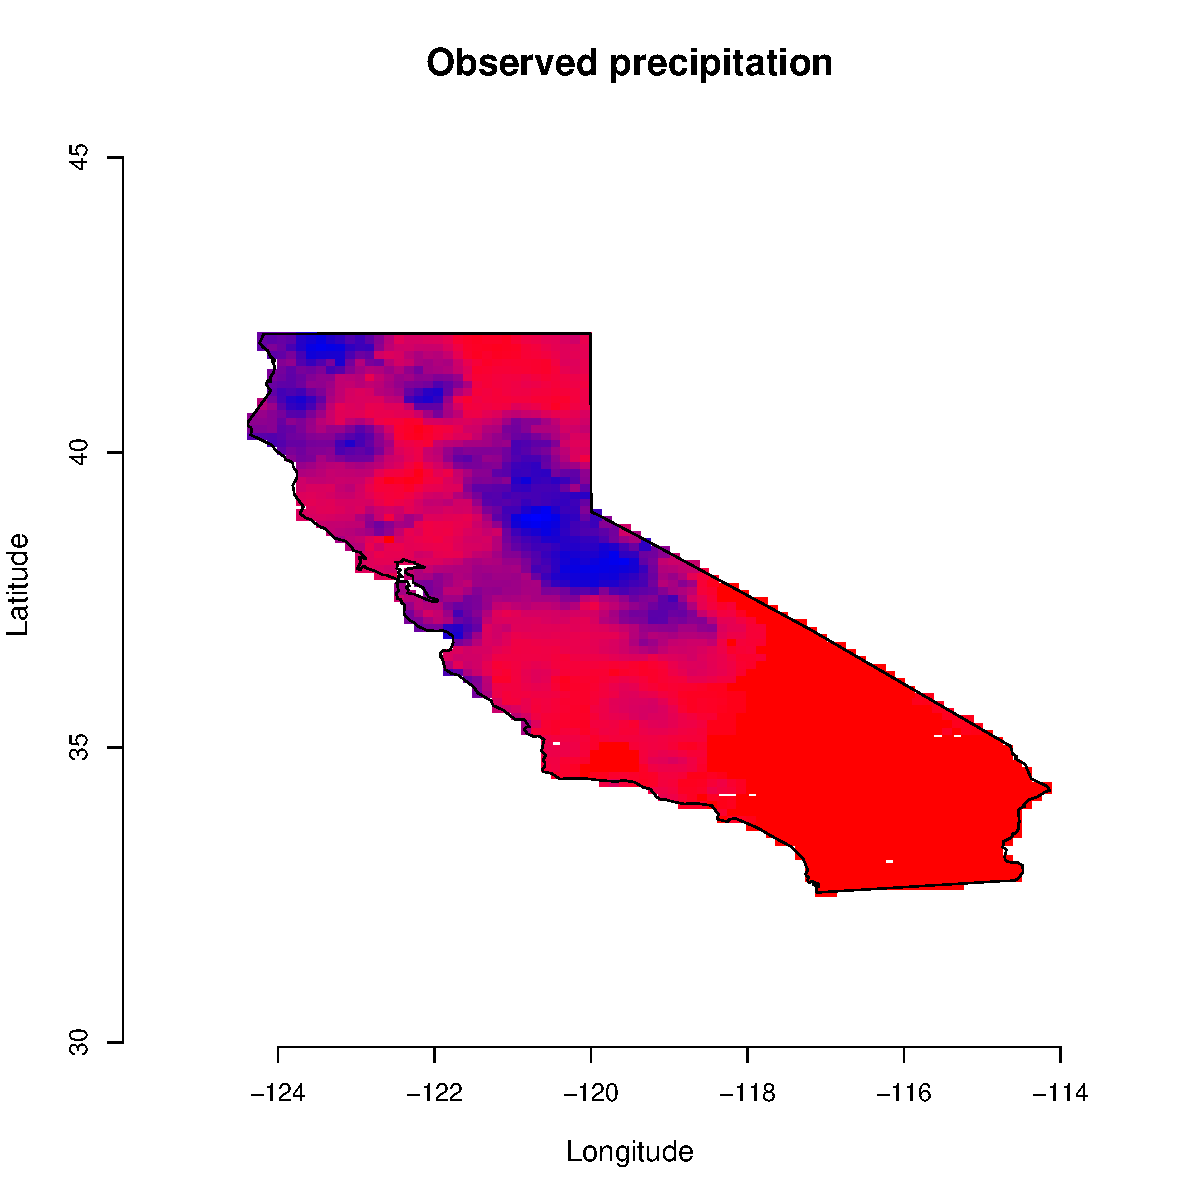
\includegraphics[scale=0.26]{/home/mickey/files/repos/stat_clim_evt_repo/figs/cal_mod_box2.pdf}
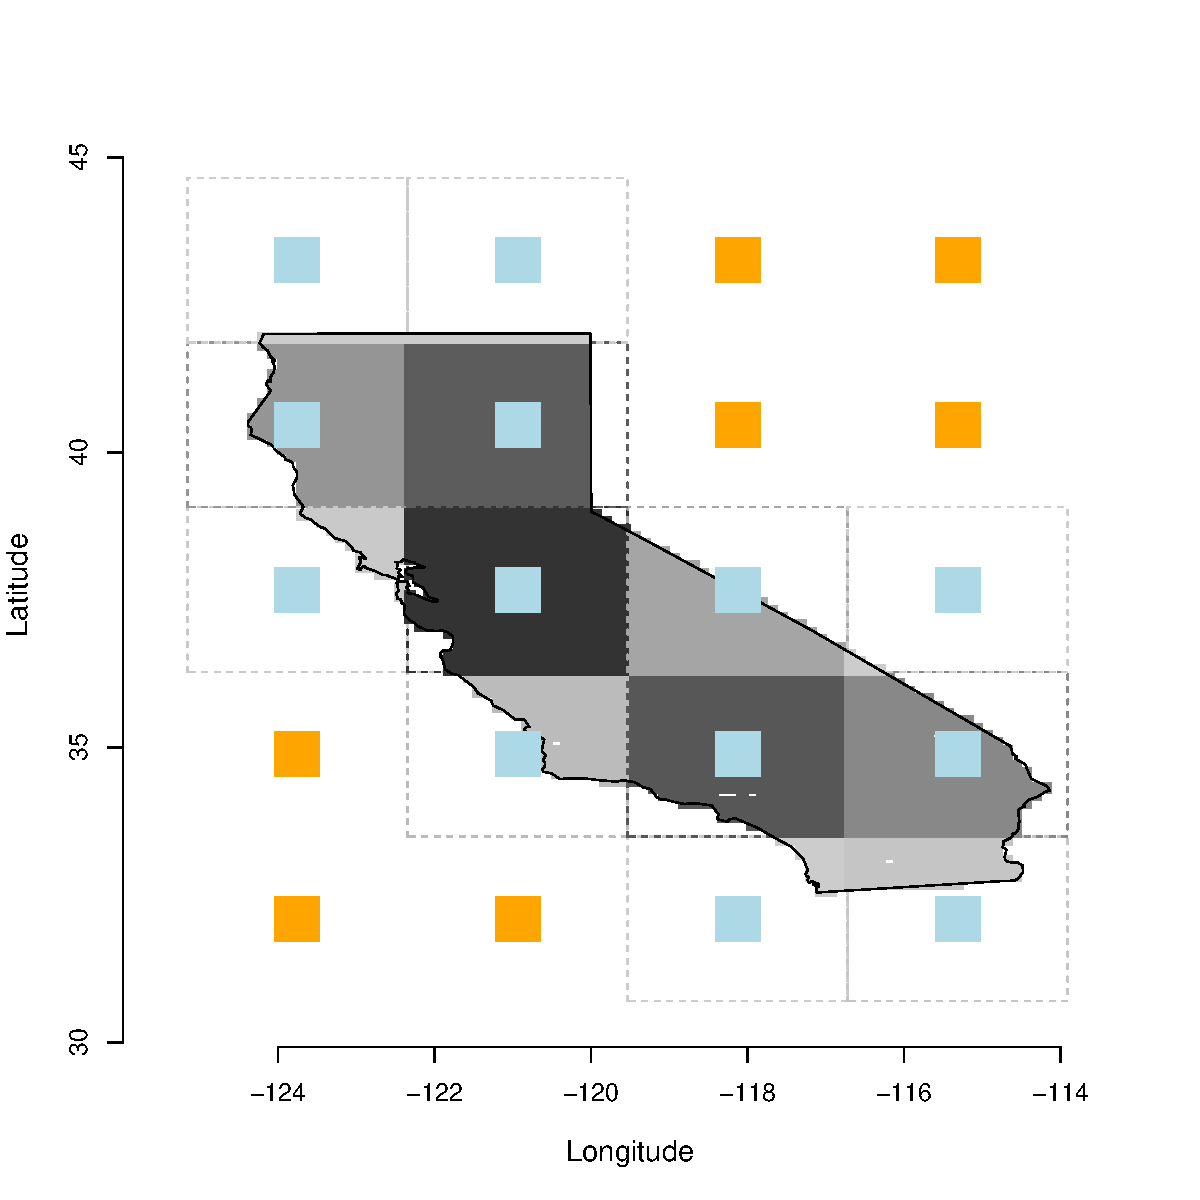
\includegraphics[scale=0.26]{/home/mickey/files/repos/stat_clim_evt_repo/figs/cal_mod_box3.pdf}
\end{center}
\caption{Left: CanCM4 simulation locations. Center: Observation locations. Right: method for computing weighted sum or average for CanCM4 to make values comparable with observations. The data shown are from a single day in January.}
\end{figure}
 
\section{Threshold exceedance model}
\label{thresh}

Under some mild assumptions, for random variable $X$ and for large enough $u$, the distribution of $X-u$ (the exceedance), conditional on $X>u$ is approximately
\begin{align}
P(X-u\leq y|X>u) \approx H(y) = 1 - \left(1+\frac{\xi y}{\sigma}\right)^{-1/\xi} \label{gpapprox}
\end{align}
defined on $\{y:y>0~\mathrm{and}~(1+\xi y/\sigma) >0\}$. $H(y)$ is the distribution function for a generalized Pareto random variable with shape paremeter $\xi\in\R$ and scale $\sigma>0$.

Let $X_1,\ldots,X_n$ be a sequence of i.i.d. random variables and $u$ be a high threshold. Define $Y_i=X_i-u$ for $X_i>u$ be the $k$ exceedances. The likelihood of $(\xi,\sigma)$ is derived from (\ref{gpapprox}) as
\begin{align}
L(y_1,\ldots,y_k;\sigma,\xi)=\sigma^{-k}\sum_{i=1}^k\left(1+\frac{\xi y_i}{\sigma}\right)_+^{-1/\xi-1} \label{gplike}
\end{align}
where $z_+=\max(z,0)$. This provides the basis for an extreme value analysis.

In many cases, the assumption of independence in observations may be too strong. When we have dependent random variables, which is likely the case in a time series, we employ a declustering scheme to obtain independent clusters, discussed in section \ref{index}
\bigskip

% \begin{align*}
% P(X-u\leq y|X > u) &= P(X\leq y+u|X > u) \\
%  &= 1 - P(X> y+u|X > u) \\
%  &= 1 - \frac{P(X>y+u, X>u)}{P(X>u)}  \\
%  &= 1 - \frac{P(X>y+u)}{P(X>u)}  \\
%  &= 1 - \frac{1-P(X-u \leq y)}{P(X>u)}  \\
% \Rightarrow P(Y\leq y) = P(X-u\leq y) &= 1-P(X>u)\left(1 - P(X-u\leq y|X>u)\right) \\
%  &= 1-\zeta\left(1+\frac{\xi y}{\sigma}\right)^{-1/xi} \\
% \end{align*}
% where $\zeta=P(X>u)$.
% \bigskip

\subsection{Hierarchical model}
\label{hier}

Suppose we have $R$ replicates or computer simulations, each with $n_i$ observations, for $i=1,\ldots,R$. Let $X_{ij}$ denote the $j$th observation in replicate $i$. We assume
\[ X_{ij} \sim F_i,~~~~~i=1,\ldots,R,~~~~~j=1,\ldots,n_i \]
and all $X_{ij}$ are mutually conditionally independent. From (\ref{gplike}), we deriv

For a fixed $u$ and each $i$, define the following sets:
\[ A_i = \{j:x_{ij}\leq u\},~~~ A_i^c = \{j: x_{ij}>u\} \]
where $|A_i|=n_i-k_i$ and $|A_i^c|=k_i$ with $k_i$ being the number of exceedances in replicate $i$. We define our exceedances as
\[ y_{ij} = (x_{ij}-u)\cdot \ind_{(j \in A_i^c)} \]
so that all observations not exceeding $u$ are marked as $0$. Let $\m{y}_i=(y_{i,1},\ldots,y_{i,n_i})^\top$ and $\m{y}=(\m{y}_1^\top,\ldots,\m{y}_R^\top)^\top$.
\bigskip

The likelihood is given by
\begin{align}
L(\m{y}; \m{\sigma}, \m{\xi}, \m{\zeta}) &= \prod_{i=1}^R f_{Y_i}(\m{y}_i|\sigma_i,\xi_i,\zeta_i) \nonumber \\
&= \prod_{i=1}^R\left[\prod_{j\in A_i} F_{X_i}(u) \times \prod_{j\in A_i^c} f_{X_i}(y_{ij}+u)\right] \nonumber \\
&\approx \prod_{i=1}^R\left[\prod_{j\in A_i} F_{X_i}(u) \times \prod_{j\in A_i^c} [1-F_{X_i}(u)]h(y_{ij}|\sigma_i,\xi_i)\right]~~~~~\mathrm{(approximation~(\ref{gpapprox}))} \nonumber \\
&= \prod_{i=1}^R\left[\prod_{j\in A_i} (1-\zeta_i)\times \prod_{j\in A_i^c} \frac{\zeta_i}{\sigma_i}\left(1+\xi_i\frac{y_{ij}}{\sigma_i}\right)_+^{-1/\xi_i-1}\right]~~~~~\mathrm{(\zeta_i=1-F_{X_i}(u))} \nonumber \\
&= \prod_{i=1}^R\left[(1-\zeta_i)^{n_i-k_i}\zeta_i^{k_i}\prod_{j\in A_i^c}\frac{1}{\sigma_i}\left(1+\xi_i\frac{y_{ij}}{\sigma_i}\right)_+^{-1/\xi_i-1}\right] \label{biglike}
\end{align}

Note that the parameters describing the tail of $F_i$ (i.e. $\xi_i,\sigma_i$) depend only on those observations which exceed $u$. The parameter $\zeta_i=P(X_i>u)$, which is necessary for calculating return levels (section \ref{return}), is based only on the number of exceedances.

We complete the hierarchical model formulation by specifying the following priors:
\begin{align}
\xi_i|\xi, \tau^2  &\sim Normal(\xi, \tau^2) \nonumber \\
\sigma_i|\alpha, \beta &\sim Gamma(\alpha, \beta) \nonumber \\
\zeta_i|\zeta, \eta &\sim Beta(\zeta\eta, (1-\zeta)\eta) \nonumber \\
 \label{priors} \\
\xi &\sim Normal(m, s^2)&  &\tau^2 \sim Gamma(a_\tau, b_\tau) \nonumber \\
\alpha &\sim Gamma(a_\alpha, b_\alpha)&  &\beta \sim Gamma(a_\beta, b_\beta) \nonumber \\
\zeta &\sim Beta(a_\zeta, b_\zeta)&  &\eta \sim Gamma(a_\eta, b_\eta) \nonumber
\end{align}

\section{Extremal Index}
\label{index}

The previously described model relies on an assumption of independence which is unrealistic for a time-series. When there is dependence between the random variables, the extremes are related according to the so-called extremal index, denoted by $\theta$.

Ferro and Suveges propose ways for estimating $\theta$. It was our experience that the likelihood provided by Ferro worked better in estimating $\theta$ in a hierarchical setting than the likelihood proposed by Suveges. 

Copy details from the other notes.

\section{De-trending}
\label{anomaly}

Each time-series is ``de-trended'' prior to declustering and parameter estimation. For each time-series, we fit a dynamic linear model (DLM) with annual and semi-annual periods. From the DLMs we obtain a smoothed version of the time-series, and then take the difference between the original series with the smoothed version. The differences are called the anomalies and the subsequent analyses are performed on them.

Each analysis is confined to a specific season, either winter or summer. Winter months are defined as December, January, and February, and summer months are June, July, and August. After de-trending based on the whole time-series, we remove all observations that do not belong to the season of interest. The remaining observations are concatenated so that, for example in winter, 28 February is followed immediately by 1 December.

Include picture of smoothed DLM


\section{Return levels}
\label{return}

The $m$-observation return level is
\begin{align}
x_m = u +\frac{\sigma}{\xi}\left[\left(m\zeta\theta\right)^\xi-1\right] \label{rl}
\end{align}

The posterior mean for $\theta$ is used, not samples, when obtaining the return levels.


\section{Results}
\label{results}

\begin{figure}
\begin{center}
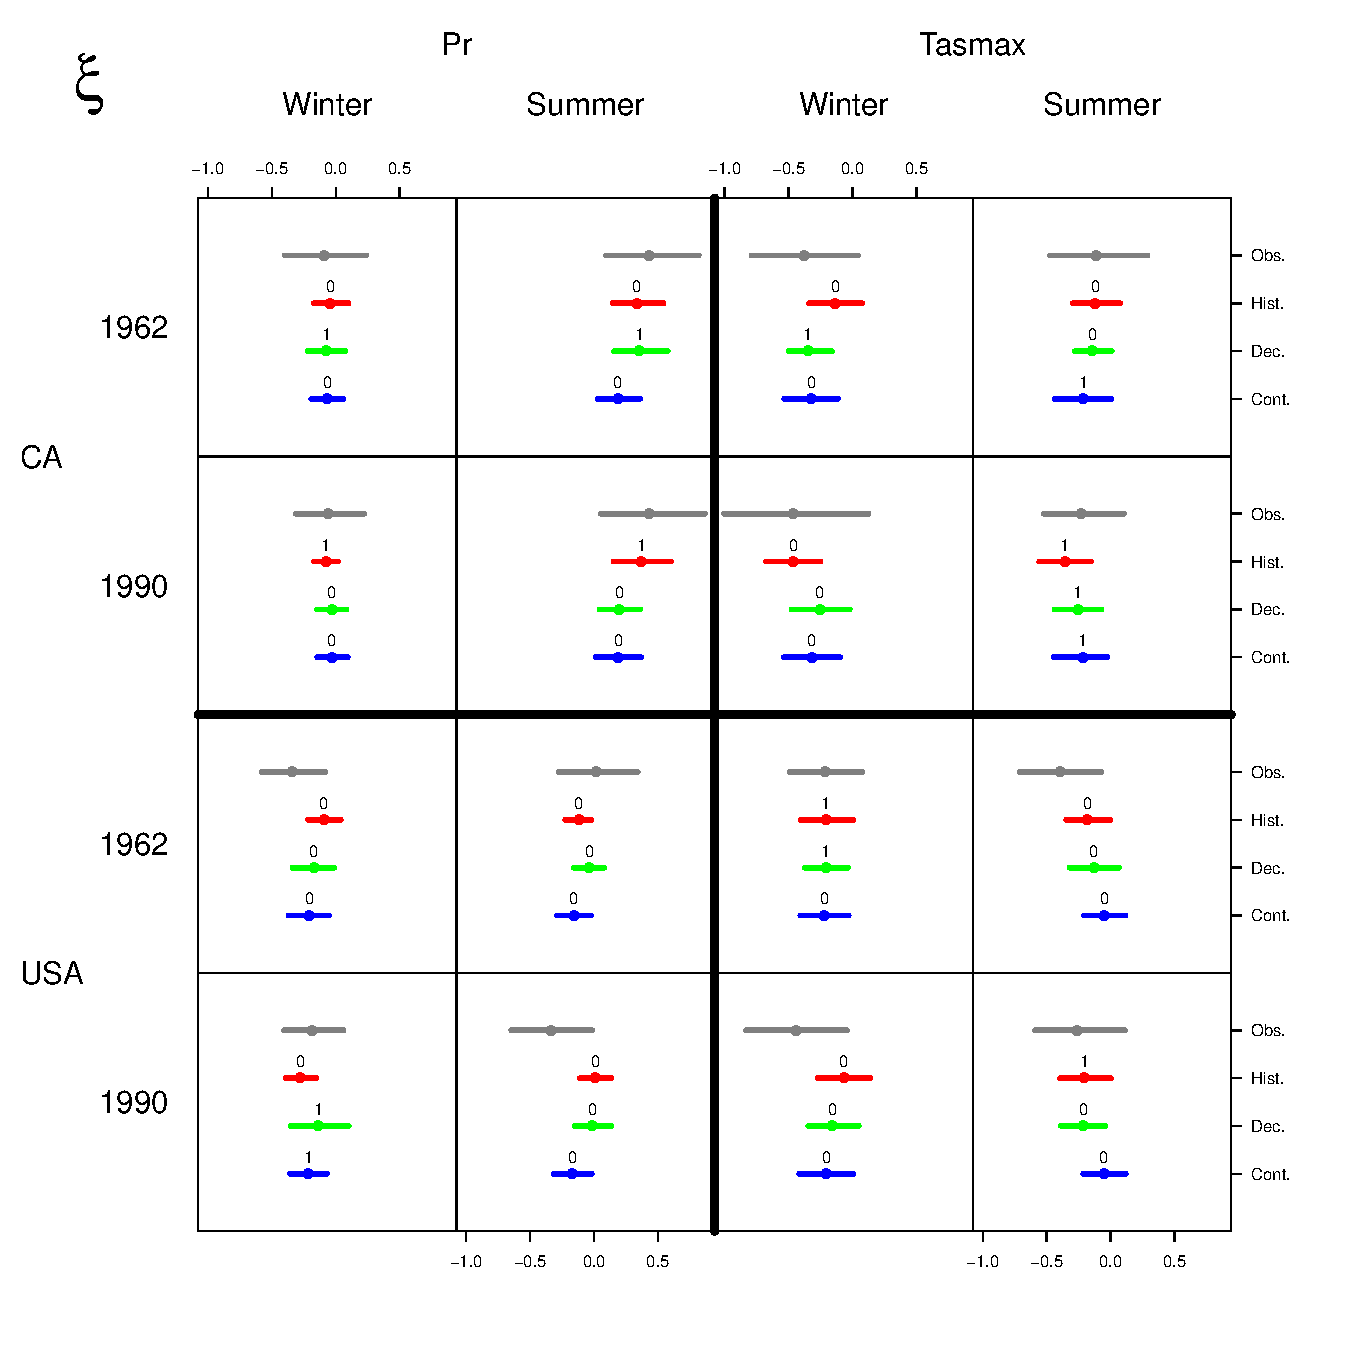
\includegraphics[scale=0.5]{figs/shape.pdf}
\end{center}
\end{figure}

\begin{figure}
\begin{center}
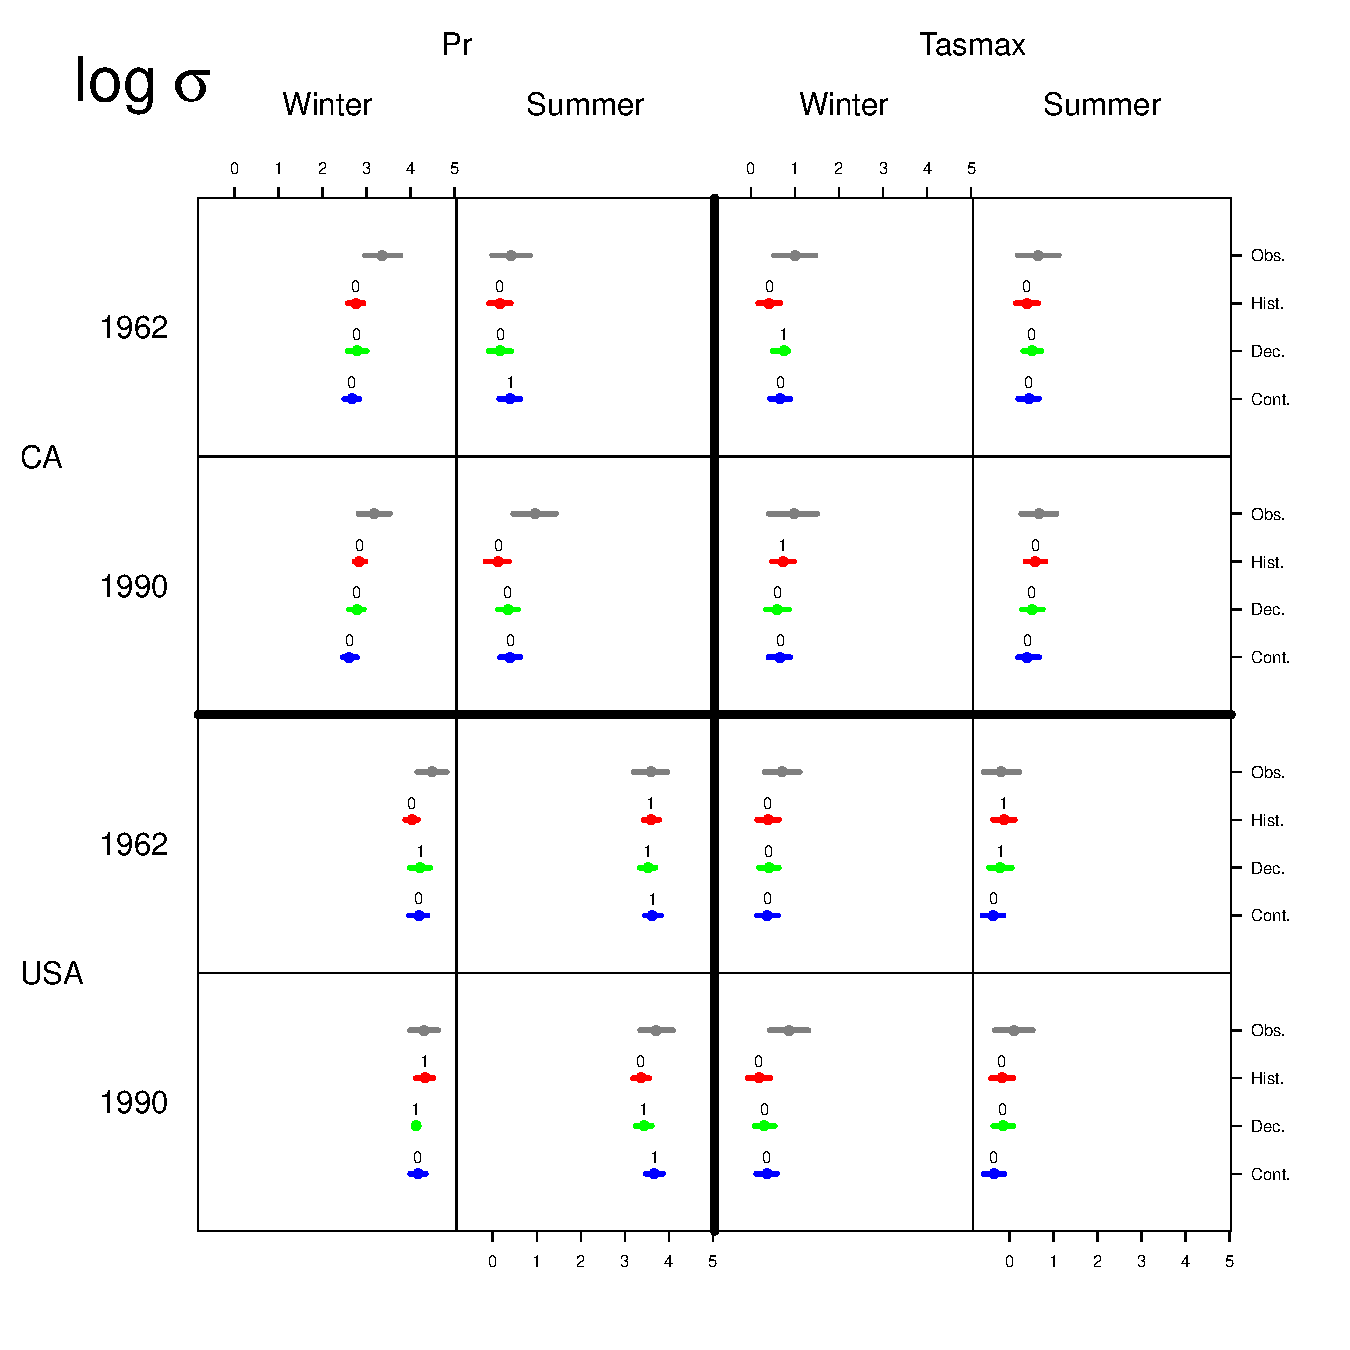
\includegraphics[scale=0.5]{figs/log_sigma.pdf}
\end{center}
\end{figure}

\begin{figure}
\begin{center}
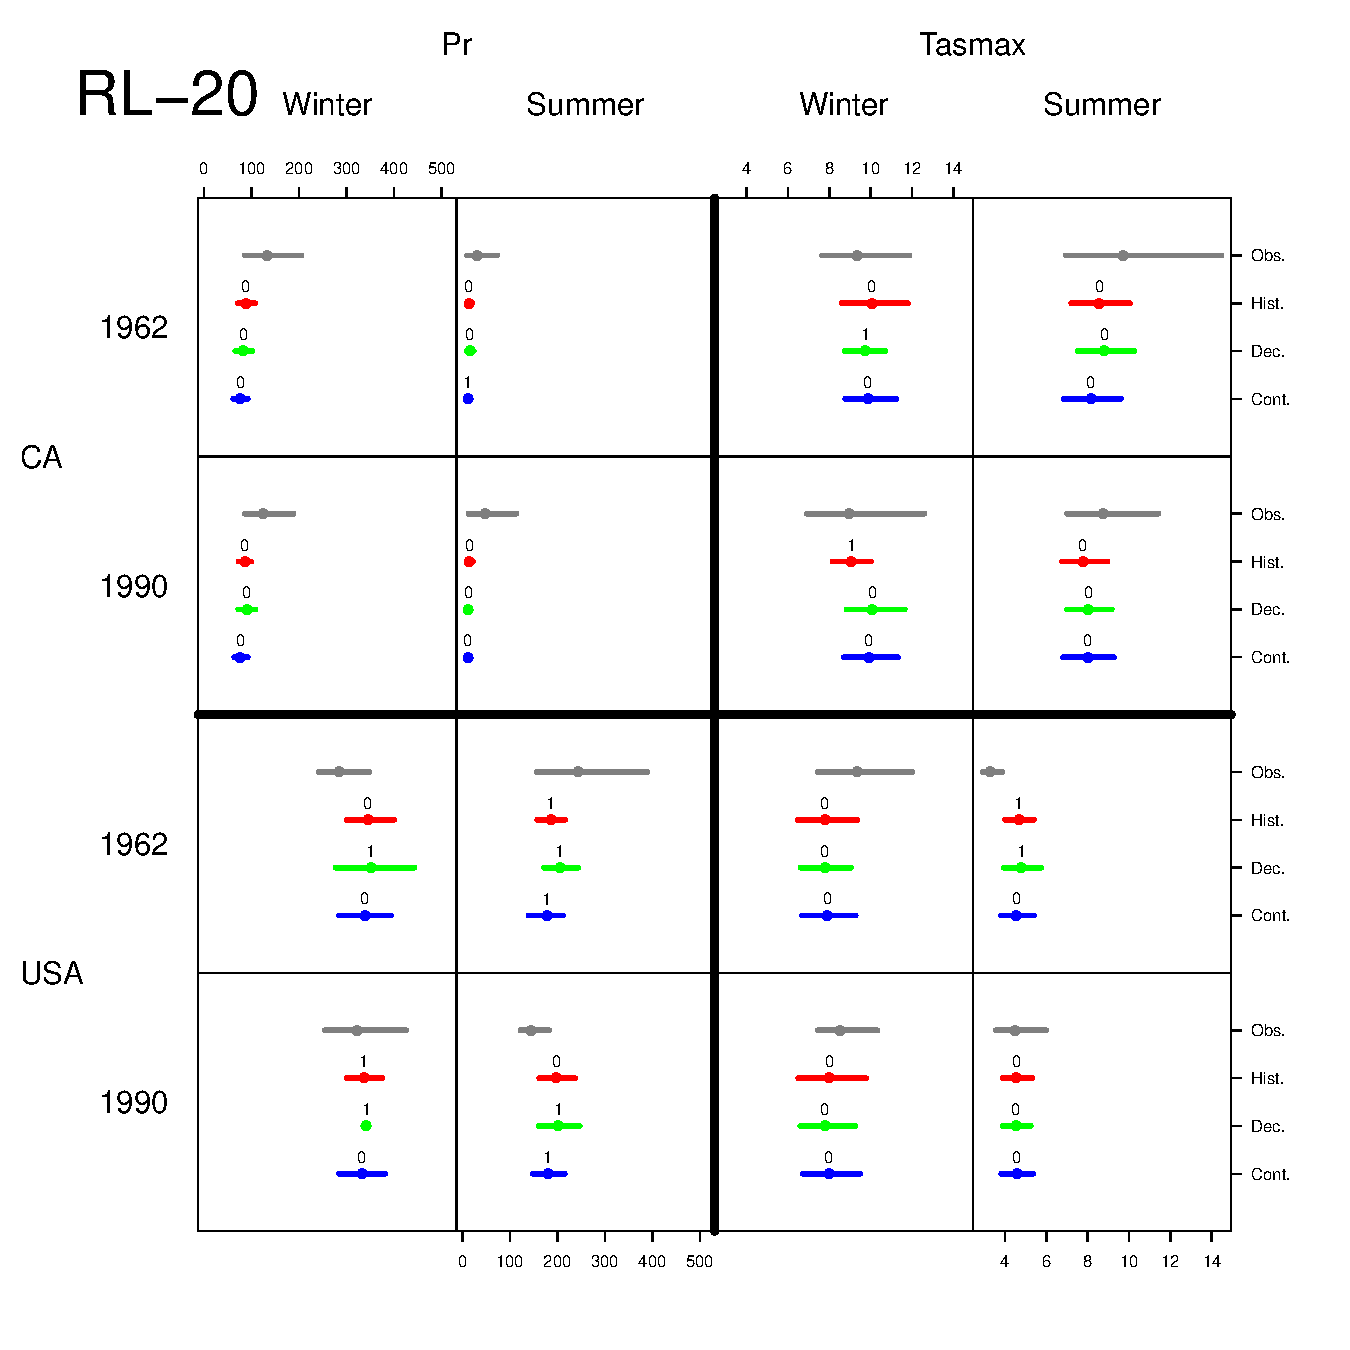
\includegraphics[scale=0.5]{figs/rl20.pdf}
\end{center}
\end{figure}

\begin{figure}
\begin{center}
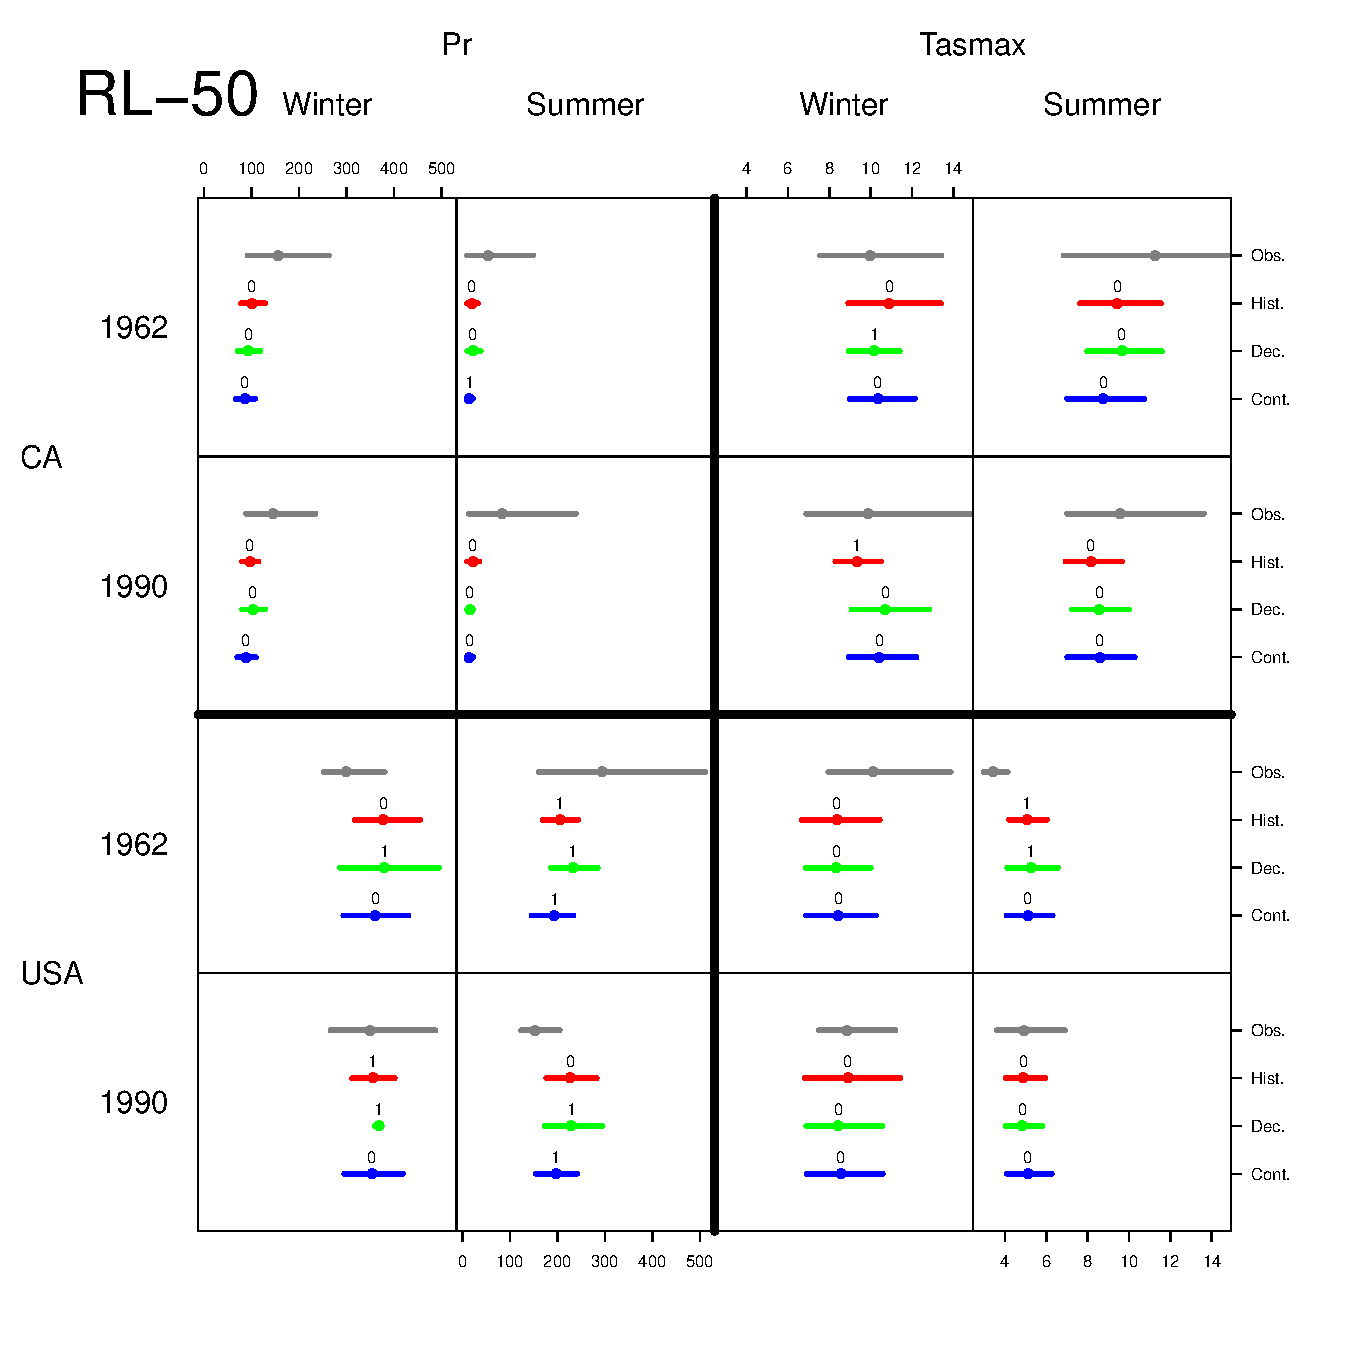
\includegraphics[scale=0.5]{figs/rl50.pdf}
\end{center}
\end{figure}

\section{Discussion}
\label{discussion}





\end{document}
